\chapter{Measuring Tool}
A critical part of performance testing is to ensure as few variables as possible change during each run of the experiment. This generates more consistent results, and allows easier comparison between test runs.\\
In a typical science experiment setup, the variables are separated into dependent, independent, and controlled variables. The dependent variables for this testing are of course the throughput and latency numbers that result from performance benchmarking, as well as the CPU usage of the applications during the test runs. For independent variables, the implementation of the application: in node.js or Java. The exact same tests are running against different implementations. Besides these variables, everything else is controlled and kept static.\\


\section{Average Response time & Throughput}
The Average Response Time takes into consideration every round trip.The resulting metric is a reflection of the speed of the web application being tested – the best indicator of how the server is performing from the users’ perspective. The Average Response Time includes the delivery all resource being used. Thus, the average will be significantly affected by any slow components. For example,  geographic locations can have small impact on response times if the end user is thousands of miles away from the server.\\
In the thesis response time is measured in three different places as you can see from figure \ref{measure-rt} , response time is measured from three different places. The first measuring is done by load generator which records the true end-to-end time and throughput. The second checkpoint is the response time retrieved from log stash which present the round trip from router. Last measuring spot is inside server itself. It reflects the round trip of a query in database. The end-to-end measuring result is used in the final performance analysis while the others served as tool to determine where is the bottleneck of the performance test is. \\

\begin{figure}[h]
	\centering
	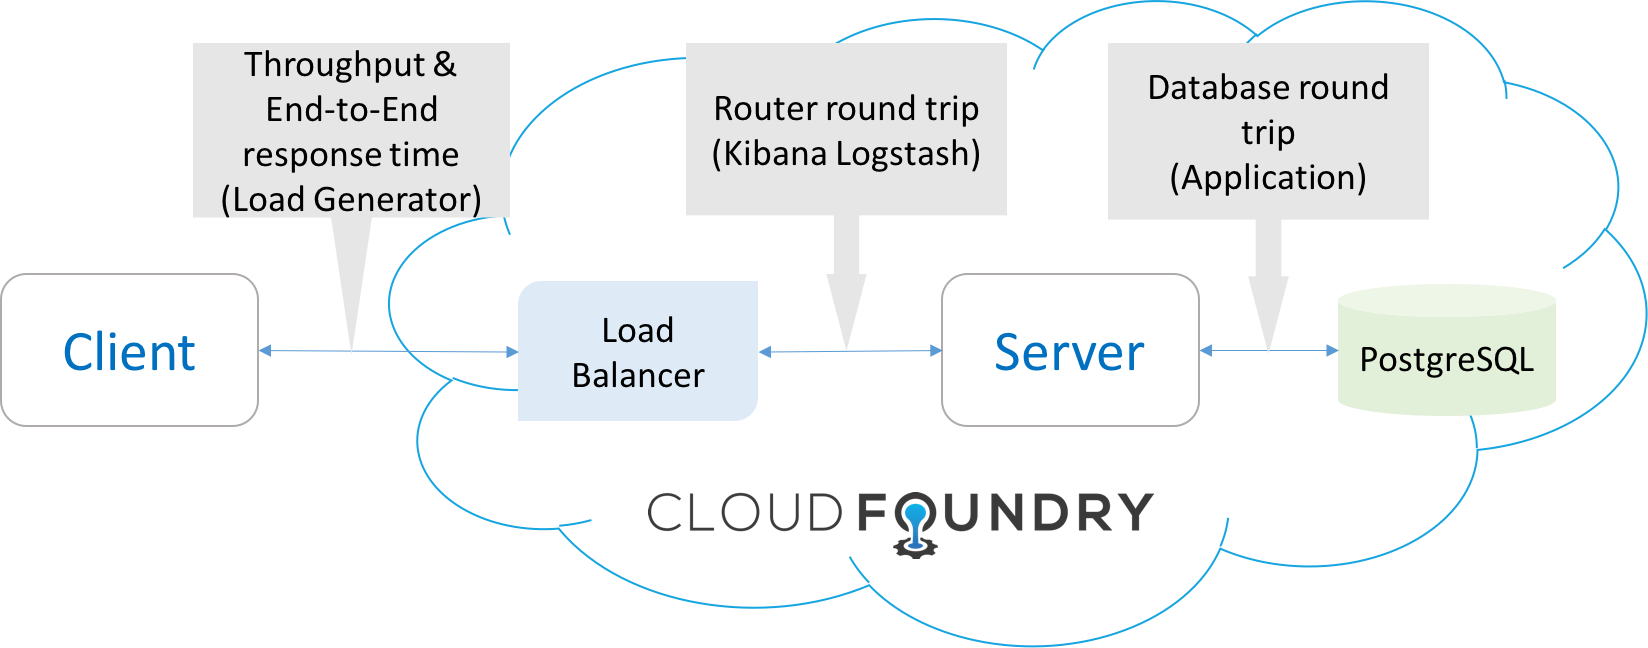
\includegraphics[width=12cm]{measure-rt}
	\caption{Measure response time three different places}
	\label{measure-rt}
\end{figure}

Throughput is the measurement of bandwidth consumed during the test. It shows how much data is flowing back and forth from servers. The requests made to the server in the thesis do not consume data of any significant size, like images. Therefore the throughput would directly reflect successfully handled amount of requests during the load testing. \\
\subsection{Recording with Load Generator and its limitations}
 In chapter \ref{load generator}, it is discussed how the load generator drives loads. It carries another duty to record the end-to-end response time fro each request. Together with response time it also stores the correlation id and start time for each request. The data is first saved in an array and insert into database at the end of load generating. \\
 However, these information are not enough. It would also be great to know the response time is resulted from which test settings, like how many application instances or how many parallel requests are sent. Therefore these information is given to the load generator and saved along with response time. Since the load generator in this thesis is only a worker, it has no API to call with given parameters. All the information external from the generator has to be given as start command. However, in cloud foundry, one application has only one start command. This means the generator should be pushed to the cloud foundry every time the parameter is changed. A small shell script is written to fulfill the task of pushing owing to the limited time frame of the thesis. Table \ref{entities stored from load generator} shows which raw data are stored. \\
 
 It is easy to scale load generator according to what one needs. On the other hand, it also means the generator has to stay stateless, which causes some extra work. For example, the same tests may be carried out in several rounds. The result of different round should be saved to compare with each other. Making \textit{test round }a automatically incremented data type is what first comes to mind. Yet it can't be defined like that when there are more than one instance of the generator running. This parameter is hence manually given for every new round of test.\\
 
\subsection{Retrieving data from Logstash and its limitations}
Application involves multiple components to accomplish one little task. Performance test can very easily hit limit of one of the components and converting the test of application into test of router or database. On account of avoiding such cases, finding and ruling out the bottleneck of all the components are carried out after the application is implemented. \\
Network is one of the major causes of bottleneck. Is the router capable of taking in so many requests? The best way is to get the response time from router. Although router is not accessible as a component to the developers,\ac{ELK}\footnote{Elasticserch, Logstash and Kibana \citep{ELK}} is integrated into cloud foundry at SAP. Router response time is logged automatically for every request. The logs produced in the application are saved in Logstash \footnote{Logstash \citep{Logstash}}and visualized in Kibana \footnote{Kibana \citep{Kibana}}. \\ 
However, in order to compare the router response time with end-to-end response time, just see the results from visualization in Kibana is not enough. To investigate what causes an exceedingly long response time, one has to seek out the precise request and do the comparison. Kibana's visualization is pretty but more convenient would be directlt comparing the figures from Logstash. To retrieve the results, a simple node application is written. It sends a json query to the logstash and then parse the query results and sort out the response time logged by router. Following that the statistics are stored into a database.\\
Of course, the result from query into Logstash can be very large and takes some time. More strangely the logs appeared to be missing. Especially when the load is large. Only ten percent of the requests are retrieved from Logstash. After ruling out there is anything wrong with the application that retrieves the result, it is observed that the logs are retrieved always retrieved as bundles of 1000 requests which can be clearly seen from Kibana. After inquiring the colleagues responsible for monitoring,  it turns out there is quota for logs. They don't come unlimited. One can only get a certain total of logs preserved per hour or per day.\\
In spite of incomplete information from Logstash, the comparison from the retrieved data shows the router has no performance bottleneck, at least not at the scale this thesis is aiming for. This leads to the realization of the HAProxy limitation discussed in chapter \ref{haproxy}. 

  \subsection{Recording data inside the application and its limitations}
This would be a very simple task if there is no log limit in Logstash: just print out the response time recorded in application out and retrieve it from Logstash. With the restriction present, the data has to be saved in database. To elevate the performance of saving such large amount of entries, measures have to be taken: like using batch in Java and manipulating array to realize a bulk insert in node.js. In this thesis, the response time and correlation id are saved in an array for all the requests. Another endpoint is defined inside the application to transfer the data into database.\\
Looking into the response time from database also helps to discover where the bottleneck of database starts. Up to a certain number of parallel requests from load generator, the throughput of the application no longer increases while the average response time goes up. Comparing the response time from database, there is an exact analog from peak of end-to-end response time to the peak in the response time from database.The slower requests also require more time to get database connection. This leads to the discovery that the database used in this thesis only provides 100  concurrent connections. After all the connections are used up, concurrent quests have to wait for a free connection to query into database. \\
Another thing to be taken into consideration is the memory leak which can be caused by not transferring recorded data to database. As said above, the information got from the application help to identify the efficiency of database. After the determination of limitation, one no longer needs to analyze the data consequently forgets to call the endpoint and transfer the data to database. As a result, the array will accumulate, grow into a considerable size and cause memory. For example, correlation id is saved as 36-letter string which consumes 36 * 2 byte memory. Response time is saved as long which takes 16 byte. Putting them together, a request needs 88 byte memory to store the response information. One round of load test generates 20000 to 100000 requests. which will result inoccupying up to 8 MB memory. A node application as a whole only needs maximum 100 MB to run. Therefore a switch should be built inside the application to not recording the data or there should be a central operational endpoint to clean up the array before each load testing. 
\section{CPU and Memory consumption}
In chapter \ref{cpu limitation}, it is described how cloud foundry allocate its computing resource. In this thesis, tests are conducted on different days and sometimes one notices some out of ordinary fluctuations which can be accounted for by a reallocation of computing resource. Nevertheless, CPU and memory consumption are gathered as key metrics since they are directly related to todays cloud pricing mechanism.
\subsection{Cloud Foundry CLI and its limitations}
Since the thesis has no access to the direct virtual machine in cloud foundry, it can not investigate the node. However, the Cloud Foundry command line interface provides simple command \textit{cf app <app-name>} to check the metrics. However, it is extremely annoying and inconvenient to require for the information from command line. Luckily there is a plugin, \textit{cf statistics} \footnote{cf statistics \citep{cfstatistics}},  in command line which deliver real-time metrics and statistics data. This plugin displays a terminal dashboard showing current app usage metrics/statistics. It can also stream these metrics as JSON formatted output to stdout.This tool is used in the thesis. \\
Although this tool is better than the command line, it still requires manual operation. The data gathered can not be stored into database along with other information. After all what the plugin does is only request the API of Cloud Controller  \footnote{cf statistics \citep{cloudcontroller}}from cloud foundry and gather them together. In the long run it would be advised to write one's own application which fetches the information from cloud controller's rest api. 
\subsection{Memory consumption}
The memory has double meaning in cloud foundry. One can assign a certain amount of heap memory to the application which will decide the computing resource an application can get. However, the application doesn't necessarily consume that much memory. How much memory does an application need to run? It is known at some point, when the heap reaches its maximum capacity, a full garbage collection will occur, which will bring down the size of the heap memory. Then it will start to grow again and the cycle should continue as long as the application is running. An application with no memory leaks should continue this cycle until the application is stopped. \\
For apps deployed on Cloud Foundry, one way to find out if it has enough native memory to run the application is to let it run under load until the first full garbage collection occurs. The total used memory of the container will continue to grow until this first garbage collection occurs. After that, the memory utilization of the container will stabilize and will not grow any more with sustained load. Figure \ref{memory} shows how the load test is conducted to find out how much memory the application needs to run. 

\begin{figure}[h]
	\centering
	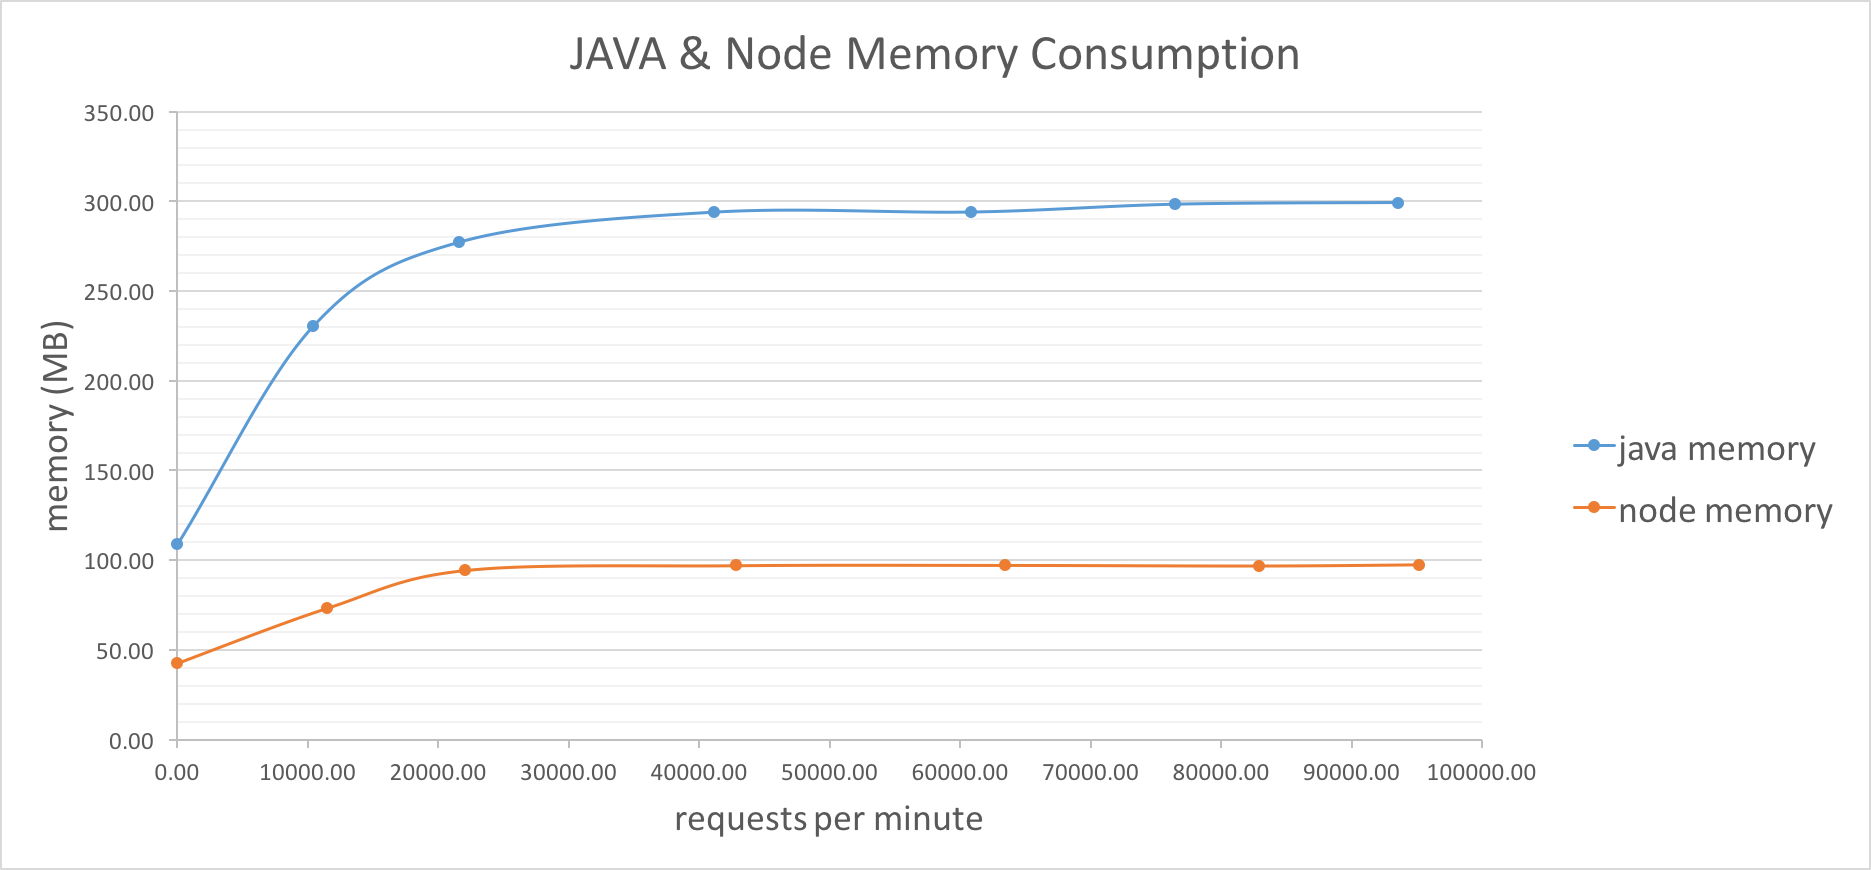
\includegraphics[width=12cm]{memory}
	\caption{Find out the memory Java and node.js applications need }
	\label{memory}
\end{figure}